\documentclass{standalone}
\usepackage{tikz,pgfplots,calc}
\usetikzlibrary{positioning,calc}
\usetikzlibrary{arrows}
\usepackage{tkz-euclide}
\usetkzobj{all}


\begin{document}
\begin{tikzpicture}[>=stealth', thick]


    \node [label = below: Iris setosa] (n1) at (0, 0) {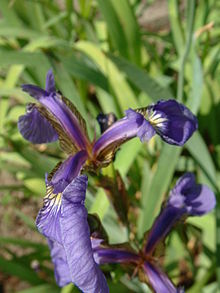
\includegraphics[height = 100pt]{iris1.jpg}};
    \node (n2) [anchor = west, right = -5pt of n1.east, label = below: Iris versicolor] {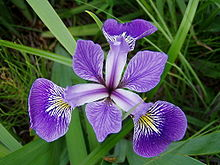
\includegraphics[height = 100pt]{iris2.jpg}};
    \node (n3) [anchor = west, right = -5pt of n2.east, label = below: Iris virginica] {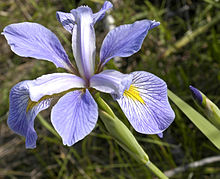
\includegraphics[height = 100pt]{iris3.jpg}};
    % \node at (\xx + 2.2, \xy + .2) {$=$};
    % \node at (\xx+5.5, \xy + .2) {\includegraphics[height = 100px]{digit7.png}};
    % \node at (\yx, \yy + .2) {$\mathbf{y}$};
    % \node at (\xx + .2, \yy - .2) {$\mathbf{z}$};
    % \node at (\xx, -.25) {$x_1$};
    % \node at (\yx, -.25) {$y_1$};
    % \node at (-.25, \xy) {$x_2$};
    % \node at (-.25, \yy) {$y_2$};
    % \node [rotate = -23] at (.5*\xx + .5*\yx, .5*\xy + .5*\yy + .3) {\textcolor{blue}{$\mathbf{\|\mathbf{x - y}\|_2}$}};
    % \draw [dashed] (y) --(\yx, 0);
    % \draw [dashed] (xy) --( 0, \yy);
    % \draw [blue, thick] (x) -- (y) ; 
    % \draw [red, thick] (x) -- (xy); 
    % \draw [red, thick] (y) -- (xy); 
    % \node at (.5*\xx + .5*\yx, \yy + .3) {\textcolor{red}{${|x_1 - y_1|}$}};
    % \node [rotate = -90, blue] at (\xx+.3, .5*\xy + .5*\yy) {\textcolor{red}{$|x_2 - y_2|$}};
    % \node [red] at (.5*\xx + .5*\yx, .5*\xy + .5*\yy + 1.7) {\textcolor{red}{$\mathbf{\|\mathbf{x - y}\|_1 = |x_1 - y_1| + |x_2 - y_2|}$}};
    % \draw 
    % \draw 


\end{tikzpicture}
\end{document}